\chapter[Introdução]{Introdução}

\chapter[Referencial Teórico]{Referencial Teórico}

Esta seção apresenta o referencial que embasa este trabalho, de forma a demonstrar o resultado da revisão de literatura feita. O referencial teórico é o meio em que o autor do trabalho demonstra o seu conhecimento sobre uma determinada área de estudo (teorias, vocabulários, variáveis chave, fenômenos, métodos e história) \cite{randolph2009}.

O referencial teórico é composto dos seguintes assuntos: \textit{End User Development}.


\section{\textit{End User Development}}

\textit{End User Development} (Desenvolvimento por usuário final) é um modelo de desenvolvimento de software onde o usuário final é o principal responsável pela construção do software. \citeonline{lieberman2006} define o \textit{End User Development} (EUD) como um conjunto de métodos, técnicas e ferramentas que permitam aos usuários de sistemas de software, que agem como desenvolvedores de software não profissionais, em algum ponto criar, modificar ou estender um artefato de software. Dentre as motivações para este modelo de desenvolvimento, destacam-se a diversidade, a mutabilidade e a dificuldade em precisar requisitos em contextos que evoluam com uma alta frequência, o que pode levar o desenvolvimento tradicional a consumir muito tempo e atingir um alto custo. (Citar a falta de disponibilidade da TI) \cite{lieberman2006}. O EUD pode eliminar as potenciais falhas de precisão da informação inerentes ao processo de intercomunicação pessoal, e oferecer respostas mais rápidas à situações onde os requisitos mudam com uma rápida frequência. Isto é possível porque os usuários finais geralmente são especialistas no domínio em que estão inseridos e conseguem responder a mudanças nos requisitos mais rápido do que o desenvolvimento tradicional. Além disso, as características importantes que motivam esses usuários a se engajarem no desenvolvimento são o empoderamento, a velocidade de desenvolvimento, a flexibilidade e o controle sobre o software \cite{fischer2004}.

Para que o desenvolvimento seguindo este modelo possa ocorrer é necessário que existam meios para que o usuário final possa desenvolver e adaptar o software, e para tanto a tecnologia envolvida deve diminuir o esforço cognitivo necessário para a construção do software, através da aproximação conceitual entre as ações do mundo real e as do mundo da programação \cite{fischer2004}. Os usuários finais geralmente não possuem habilidades de um profissional da área de software, e também não estão interessados em construir sistemas no mesmo nível que esses profissionais, por isso é necessário que a tecnologia usada no desenvolvimento alinhe a complexidade relacionada a esta atividade com as habilidades do usuário final. Este é o principal objetivo do EUD: oferecer meios para que os usuários finais consigam desenvolver e adaptar software \cite{lieberman2006}. Desta maneira, as aplicações preparadas para o EUD devem ser, principalmente, flexíveis, fáceis de se entender, de se usar, e de se ensinar \cite{lieberman2006}. A preocupação com a tecnologia usada neste modelo de desenvolvimento, mais especificamente na parte das linguagens de programação e aplicações de desenvolvimento, é a relação escopo de aplicação versus esforço de aprendizagem. A figura 1 ilustra a relação do escopo de aplicação e do custo de aprendizagem, para diferentes linguagens de programação e aplicações. Linguagens de programação mais tradicionais como C++ e JAVA oferecem a possibilidade de construção de software de uma grande variedade de domínios, porém a um alto custo associado ao esforço de aprendizagem. Outras linguagens possuem um menor esforço de aprendizagem, ao custo de uma limitação no escopo de aplicação. As linguagens ou aplicações de desenvolvimento ideais para o EUD são as que possuem um alto escopo de aplicação e um baixo esforço de aprendizagem \cite{fischer2004}. As que existem atualmente só utilizam uma pequena parte do potencial do EUD, com algumas falhas \cite{paterno2013}.


\begin{figure}[h]
	\centering
	\label{fig01}
		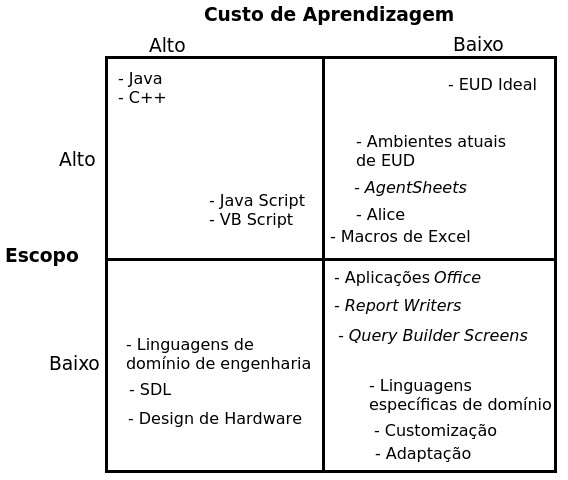
\includegraphics[keepaspectratio=true]{figuras/trade_off_eud_editado}
	\caption{Relação escopo de aplicação e custo de aprendizagem}
\end{figure}
\pagebreak

\citeonline{lieberman2006} classifica as atividades do usuário final em dois tipos, de acordo com uma perspectiva de \textit{design} centrada no usuário:

\begin{enumerate}
\item \textbf{Parametrização ou Customização:} São atividades que permitem o usuário escolher comportamentos, apresentações e mecanismos  alternativos, que já existem dentro de uma aplicação. Sistemas que se customizam automaticamente em resposta ao comportamento do usuário, são exemplos deste tipo de atividade.

\item \textbf{Criação e modificação de programas:} São atividades que implicam na criação ou modificação de artefatos de software. Macros e linguagens de \textit{script} são exemplos deste tipo de atividade.
\end{enumerate}

 
\chapter[Metodologia]{Metodologia}

\citeonline{gil2002} classifica as pesquisas científicas em três grandes grupos, segundo os seus objetivos gerais: exploratórias, descritivas e explicativas.

A pesquisa exploratória tem como objetivo proporcionar o aprimoramento e/ou a descoberta de idéias, a respeito de um determinado problema. Proporcionando uma maior familiaridade com o problema, esse tipo de pesquisa o torna mais explícito e contribui para a construção de hipóteses em cima do mesmo. Por conta disso, a pesquisa exploratória possui um caráter flexível em seu planejamento, e geralmente assume as formas de pesquisa bibliográfica ou estudo de caso \cite{gil2002}.

O estudo de caso consiste no estudo profundo e exaustivo de um ou mais objetos, de forma a obter conhecimento amplo e detalhado sobre o mesmo. Segundo (Citar Yin, 2001), o estudo de caso é a abordagem mais adequada para a investigação de um fenômeno em seu contexto real, onde os limites entre este fenômeno e o seu contexto não são claramente percebidos. Os propósitos do estudo de caso são \cite{gil2002}:

\begin{itemize}
\item Explorar situações de contextos reais onde os limites não estão claramente definidos.
\item Preservar o caráter unitário do objeto.
\item Descrever a situação do contexto do qual esta sendo feita a investigação.
\item Desenvolver teorias e formular hipóteses.
\item Determinar as causas de um determinado fenômeno onde a complexidade não permite o uso de levantamentos e experimentos.
\end{itemize}

O conjunto de etapas que podem ser seguidos na maioria das pesquisas classificadas como estudo de caso, bem como uma breve descrição destas etapas são apresentados a seguir \cite{gil2002}.

\begin{enumerate}
\item \textbf{Formulação do problema.}

Constitui a primeira etapa da pesquisa. O problema constitui um fato no qual se deseja aprofundar, de forma a fazer uma descrição de um determinado fenômeno, ou descobrir respostas as causas deste fenômeno. Cuidado deve ser tomado para que o tema seja passível de verificação.

\item Definição da unidade a ser estudada.
\item Determinação do número de casos
\item Elaboração do roteiro.
\item Coleta dos dados.
\item Análise dos dados coletados.
\item Elaboração do relatório.
\end{enumerate}

